\chapter{METODOLOGIA}
\label{cap3}

Neste capítulo, serão elencados os passos utilizados para o desenvolvimento do processamento sísmico realizado. Todos os passos foram realizados usando o pacote \textit{Seismic Unix}.

\section{Construindo modelo de camadas planas e aquisição}

Para o início do trabalho,  foi feito um modelo sintético para realizar o processamento sísmico. Será realizado no formato de camadas planas (\ref{fig:camadas}). Este é um modelo com três camadas com velocidades diferentes, sendo o total da distância de 6 km e uma profundidade de 2 km.

A primeira camada tem 800 metros de profundidade e possui a velocidade nesta região de 1508 m/s. A segunda camada tem 800 metros de profundidade e possui  velocidade nesta região de 1715 m/s. A última camada tem 400 metros de profundidade e possui velocidade nesta região de 1925 m/s. A Figura \ref{fig:camadas} foi gerada a partir do apêndice \ref{apendice_A}.

\begin{figure}[ht!]
	\centering
	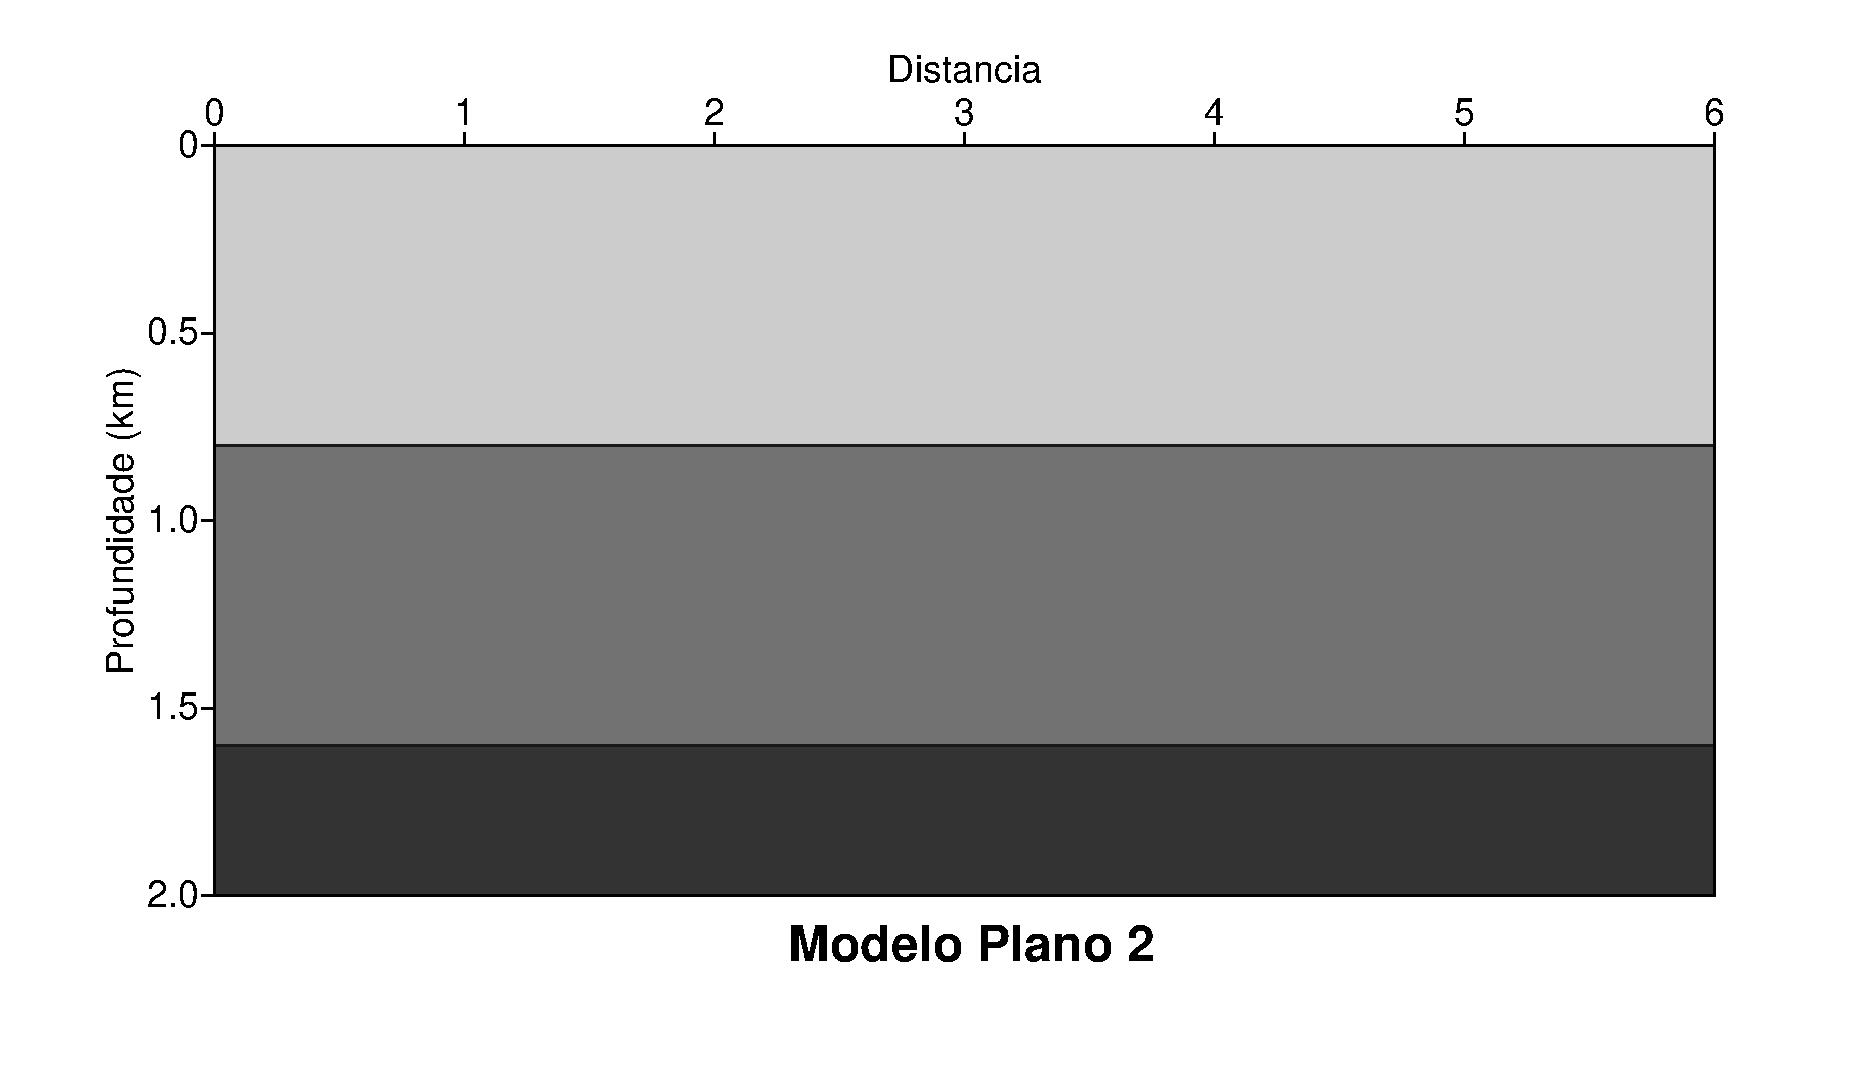
\includegraphics[width=15cm]{camadas_planas}
	\caption{Modelo 2D de camadas planas.} \label{fig:camadas}
\end{figure} 

A partir deste modelo, será feita a aquisição dos dados. Foram utilizados 40 fontes. Estas foram espaçados em 50 metros. Enquanto que foram usados 60 geofones para cada tiro, gerando um total de 2400 traços. O  intervalo de deslocamentos de geofone é entre -1475m
e 1475m. As fontes estão localizadas entre a distância de 2 km até 3.95 km, enquanto o geofone está entre 0.525km e 5.425km.
 
 Com estes resultados, será feita uma avaliação das velocidades para os CMPs e, se necessário, utilizar a correção NMO. Após estes passos, será feito o empilhamento e a migração temporal. Estes resultados serão apresentados na próxima seção.
